\begin{figure}
\centering
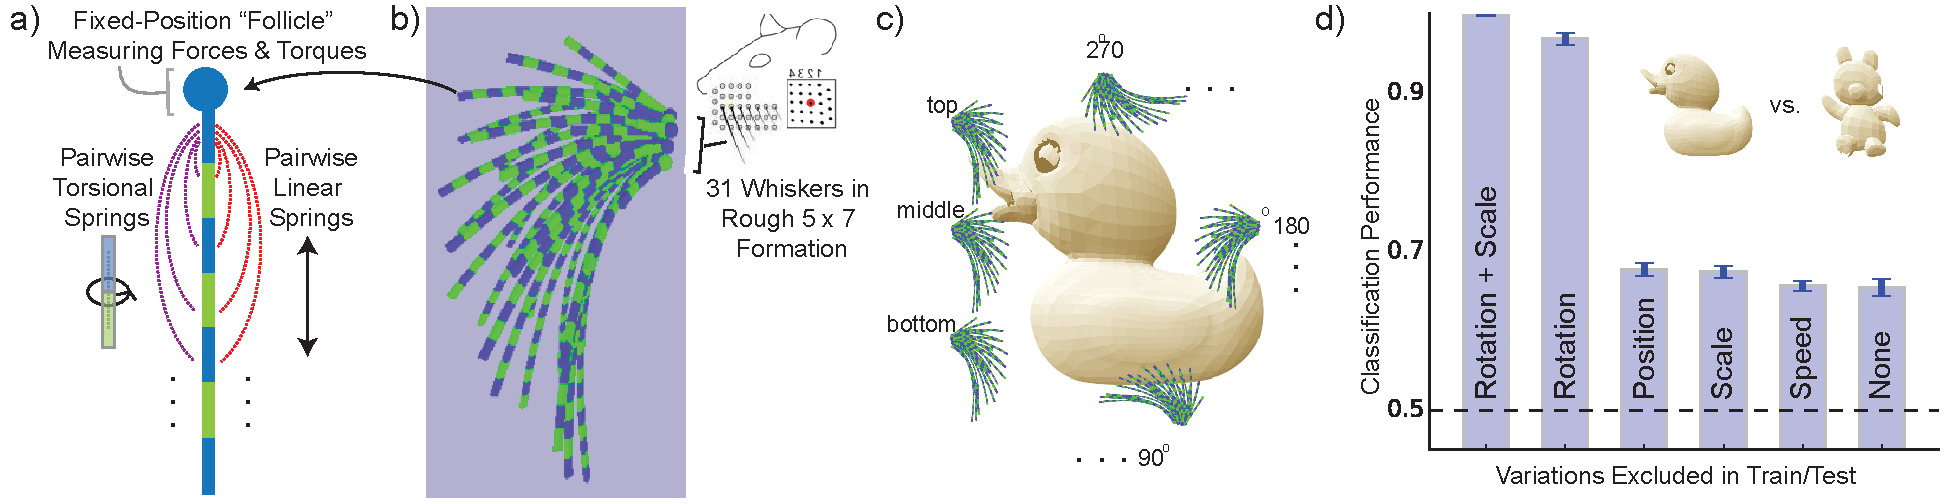
\includegraphics [width=1\linewidth]{figures/whiskers.pdf}
\vspace{-2mm}
\caption{\textbf{Dynamic Three-Dimensional Whisker Model:} \textbf{a.} We constructed an array of 31 whisker objects, arranged in a 5x7 grid (with 4 missing elements).  Whisker number, placement, length and static shape were matched to biophysical data. \textbf{b.} Each whisker element is composed of a set of cuboid objects.  The follicle cuboid has a fixed location, and is attached to movable cuboids making up the rest of the hair. Motion is constrained by linear and torsional springs between each pair of cuboid elements.  The parameters of these springs are chosen to ensure naturalistic motion of the whiskers.  \textbf{c.} During dataset construction, the whisker is brought into contact with each object at three vertical heights (top, middle bottom), at each of 4 90-degree separated attack angles, for a total of 12 swipes.  Object initial angle, size, and swipe speed vary randomly between each group of 12 swipes.  Forces and torques are recorded at the three cuboids closest to to the follicle, for a total of 18 measurements per whisker per timepoint.  \textbf{d.} ~\label{fig_whiskers}}
\end{figure}

In order to provide the similar inputs to deep neural networks as those to rodent somatosensory systems, one will need a physically accurate models for the the rodent whiskers.
In our models, we are more interested in ensuring the correctness of the mechanical details of every individual whisker.
And at the same time, we also need the simulations to be fast enough for generating a large scale dataset.
Therefore, we use Bullet~\cite{wiki:bullet} as physics engine, which is a open-source real-time physics engine used in many video games and visual effects in movies.
Meanwhile, we also need to make our model biologically accurate. So the parameters used in our model including position, curvature, and length of each whisker, are from biological static whisker model in~\cite{Towal2011}.

We use small cuboids concatenated along the longest dimension to model single whisker, where each cuboid is connected to every other cuboid in the same whisker using both linear and torsion springs.
The equilibrium points of all the springs as well as the initial positions of all cuboids are set to make the whiskers fit the required curvature.
Each cuboid is in the same shape with the length of 2mm and the number of cuboids is chosen to fit the required length for different whisker.
The bottom of whiskers will be fixed at the given positions. Except that, the motion of every cuboid is only constrained by the springs connecting to it.
Besides, there is no collision between cuboids in different whiskers or in the same whisker.
And in our simulation, we only used right whisker array.

As we are simulating the whiskers using concatenated cuboids and the dynamics of the physics engine is calculated frame by frame and kept the same between frames, we can not derive stiffness of springs between cuboids directly from dynamic related parameters of whiskers.
In addition, we need to add damping to cuboids, which means that their motion will be decayed at a fixed rate every frame. Otherwise the cuboids can not stop their motions.
As it's hard to derive those parameters from biological models, we use optimization method to find the best values maximizing the "reasonability" of the dynamic behaviors of whiskers.
Specifically, for each whisker, we construct four situations where four forces are applied to the end of that whisker for a fixed amount of time.
These four situations include pushing whisker towards the bottom, pushing whisker forward, pushing whisker forward further, and pushing whisker to its left.

For each simulatin, we simulate the process that the whisker recover to the static position after applying the force and then measure the time ($T$) needed for recovery, the distance ($S$) travelled by all cuboids between the end of applying the force and recovery, the distance ($d$) between the bottom and the end of the whisker at the end of applying the force, and the average speed ($v$) of all cuboids during the recovery.
We use hyperopt~\cite{bergstra2013hyperopt} for optimizing those hyper parameters including damping and spring stiffness. The optimization is done to every whisker independently as the hyper parameters are not shared between whiskers.
In order to reduce the number of parameters we need to optimize, we assume that within one whisker, all cuboids shares the same damping setting including linear damping and rotation damping.
Furthermore, we group the springs by the their length, which means that the spring connecting 1st cuboid and 3rd cuboid as well as the spring connecting 2st cuboid and 4th cuboid and so on will be in the same group.
For each group, we assume that the stiffness is linearly correlated with the distance between the starting cuboid of this spring and the bottom of that whisker.
This is inspired by the fact that the whisker will be thicker and stiffer at the bottom~\cite{Hartmann:2015}.
And finally, we set our loss function to be $0.025S + d + 20T - 2v$, where the coefficients are set to make each term comparable.
The hyperopt program will try to find the best hyper parameters to minimize the loss function, which means that after applying a fixed amount of force, we expect the whisker to recover as fast as we can (positive coefficients for $S$, $T$, and $v$) and also the stiffness not being so large that the whisker can not be bent (negative coefficient for $d$).

Finally, we have a whisker array consisting of 31 whiskers whose bottoms are placed on a surface of ellipsoid in a grid of $5\times7$ with some vacant positions, where the longest whisker has around 30 cuboids and shortest whisker has around 4 cuboids. 
